% !Mode:: "TeX:DE:UTF-8:Main"

\documentclass[aspectratio=169]{beamer}
\usepackage{tikz}
\usetikzlibrary{tikzlings}
\usepackage{bearwear}
\usetikzlibrary{decorations.text,fpu}

\setbeamertemplate{navigation symbols}{}

% trick taken from https://topanswers.xyz/tex?q=1989
\tikzset{
    use page relative coordinates/.style={
        shift={(current page.south west)},
        x={(current page.south east)},
        y={(current page.north west)}
    },
   tugbear/.pic= {
   \begin{scope}[scale=0.5]
    \bear\bearwear[body deco={
   \node[anchor=center] at (beartummy){
\includegraphics[scale=0.3]{tug-logo-farbe-blau}
   };
     \node[text=white, font=\sffamily\bfseries] at (beartummy) {};}]
     \end{scope}},
}

\makeatletter
\newcommand*{\slideinframe}{\number\beamer@slideinframe}
\makeatother

\newsavebox\bearbox
\savebox\bearbox{\tikz{\bear\bearwear[body deco={
   \node[anchor=center] at (beartummy){
\includegraphics[scale=0.3]{tug-logo-farbe-blau}
   };
     \node[text=white, font=\sffamily\bfseries] at (beartummy) {};}]}}
     
\begin{document}

\def\steps{350}
\begin{frame}
  \begin{tikzpicture}[
     %use page relative coordinates,     
      remember picture,
      overlay
    ]
      \node[anchor=north,inner sep=0pt] at (current page.north) 
      {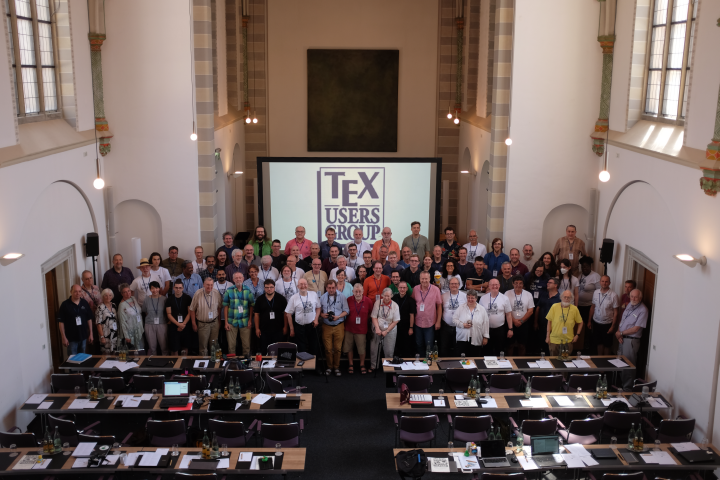
\includegraphics[width=\paperwidth]{tug2023-small}}; 
   \node[anchor=south,inner sep=0pt] at ([yshift=-3cm,xshift=-0.2cm]current page.north)
    { 
\includegraphics[]{tug-logo-farbe-blau} };      
   %\path (current page.north)--++(-0.2,-8.3)pic[] {tugbear};
   \path ([yshift=0.3cm+\fpeval{5*(0.02*sin(\slideinframe/120*4*pi))}cm]current page.south west) 
    --++ (1.5,0) pic[mouse/back,scale=0.5] {mouse}
    --++ (1,0) pic[squirrel/back,scale=0.6] {squirrel} 
    --++ (1,0) pic[rhino/back,scale=0.6] {rhino} 
    --++ (1,0) pic[koala/back,scale=0.5] {koala}
    --++ (1,0) pic[anteater/back,scale=0.5] {anteater} 
    --++ (1,0) pic[bug/back,bug/body=yellow!50!black,scale=0.5] {bug}   
    --++ (2,0) pic[chicken/back,,scale=0.5] {chicken}   
    --++ (1.2,0) pic[coati/back,,scale=0.5] {coati}
    --++ (1.2,0) pic[hippo/back,,scale=0.5] {hippo}
    --++ (1.2,0) pic[sheep/back,,scale=0.5] {sheep}
    --++ (1.2,0) pic[wolf/back,,scale=0.5] {wolf}
    ;
   
   \begin{scope}
   \path[clip](current page.south west) rectangle +(\paperwidth,0.07\paperheight);
    
    \node[anchor=north,inner sep=0pt] at (current page.north) 
      {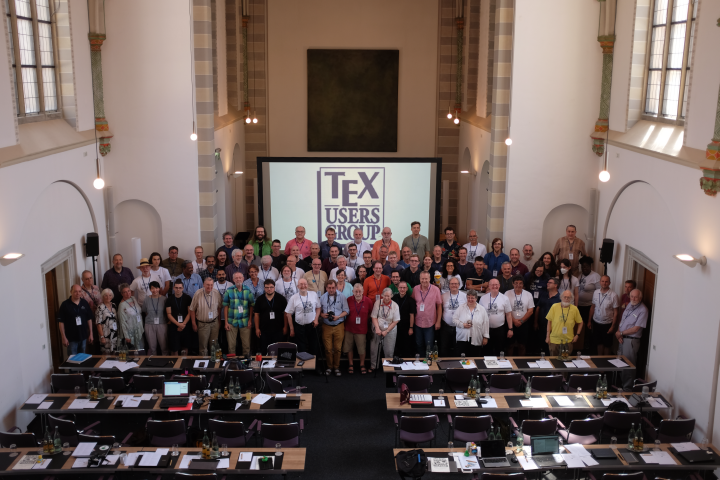
\includegraphics[width=\paperwidth]{tug2023-small}};    
   \end{scope}
   
    \path ([yshift=-0.3cm+\fpeval{5*(0.02*sin((\slideinframe+40)/120*4*pi))}cm]current page.south west) 
      --++ (1.2,0) pic[sheep/back,,scale=0.5] {sheep}
     --++ (1.2,0) pic[chicken/back,,scale=0.5] {chicken}   
     --++ (1.2,0) pic[coati/back,,scale=0.5] {coati}
     --++ (1.2,0) pic[hippo/back,,scale=0.5] {hippo}
     --++ (1,0) pic[squirrel/back,scale=0.6] {squirrel} 
    --++ (3,0) pic[rhino/back,scale=0.6] {rhino} 
    --++ (1,0) pic[koala/back,scale=0.5] {koala}
    --++ (1,0) pic[anteater/back,scale=0.5] {anteater} 
  	  --++ (1,0) pic[bug/back,bug/body=yellow!50!black,scale=0.5] {bug}  
    --++ (1.2,0) pic[chicken/back,,scale=0.5] {chicken}   
     --++ (1.5,0) pic[mouse/back,scale=0.5] {mouse} 
     ;
     
    \path (current page.north)--++(-0.5,-7.8cm)node {\scalebox{0.6}{\usebox\bearbox}};
 
      \node[white,text width=\paperwidth,font=\tiny,align=center] at ([yshift=0.25cm]current page.south) {Image by Alan Wetmore};        
   
   
  \end{tikzpicture}  
  \pause[\steps]
 
 
     
\end{frame}

\end{document}
